\section{Embedding Analysis}
\label{sec:embedding-analysis}

To understand what the learned patch representations encode, we extract two
embedding tensors per grid from the V8 and V10 models (Section~\ref{sec:architecture}):
the \textbf{pre-transformer} embedding (patch content projection $+$
learnable positional embedding, before attention) and the
\textbf{post-transformer} embedding (after the Transformer encoder mixes
information across all 100 patches). Both are $100 \times d_{\text{model}}$
tensors --- one $d_{\text{model}}$-dimensional vector per $4\times4$ patch,
arranged on a $10\times10$ grid.

\subsection{Static structure: patch norms and pairwise similarity}

For a fixed configuration, we visualize (i) the spatial map of
post-transformer embedding norms, $\|\text{emb}_i\|_2$ for each of the 100
patches, and (ii) the full $100\times100$ pairwise cosine similarity matrix
between all patches' embeddings.

\begin{figure}[htbp]
  \centering
  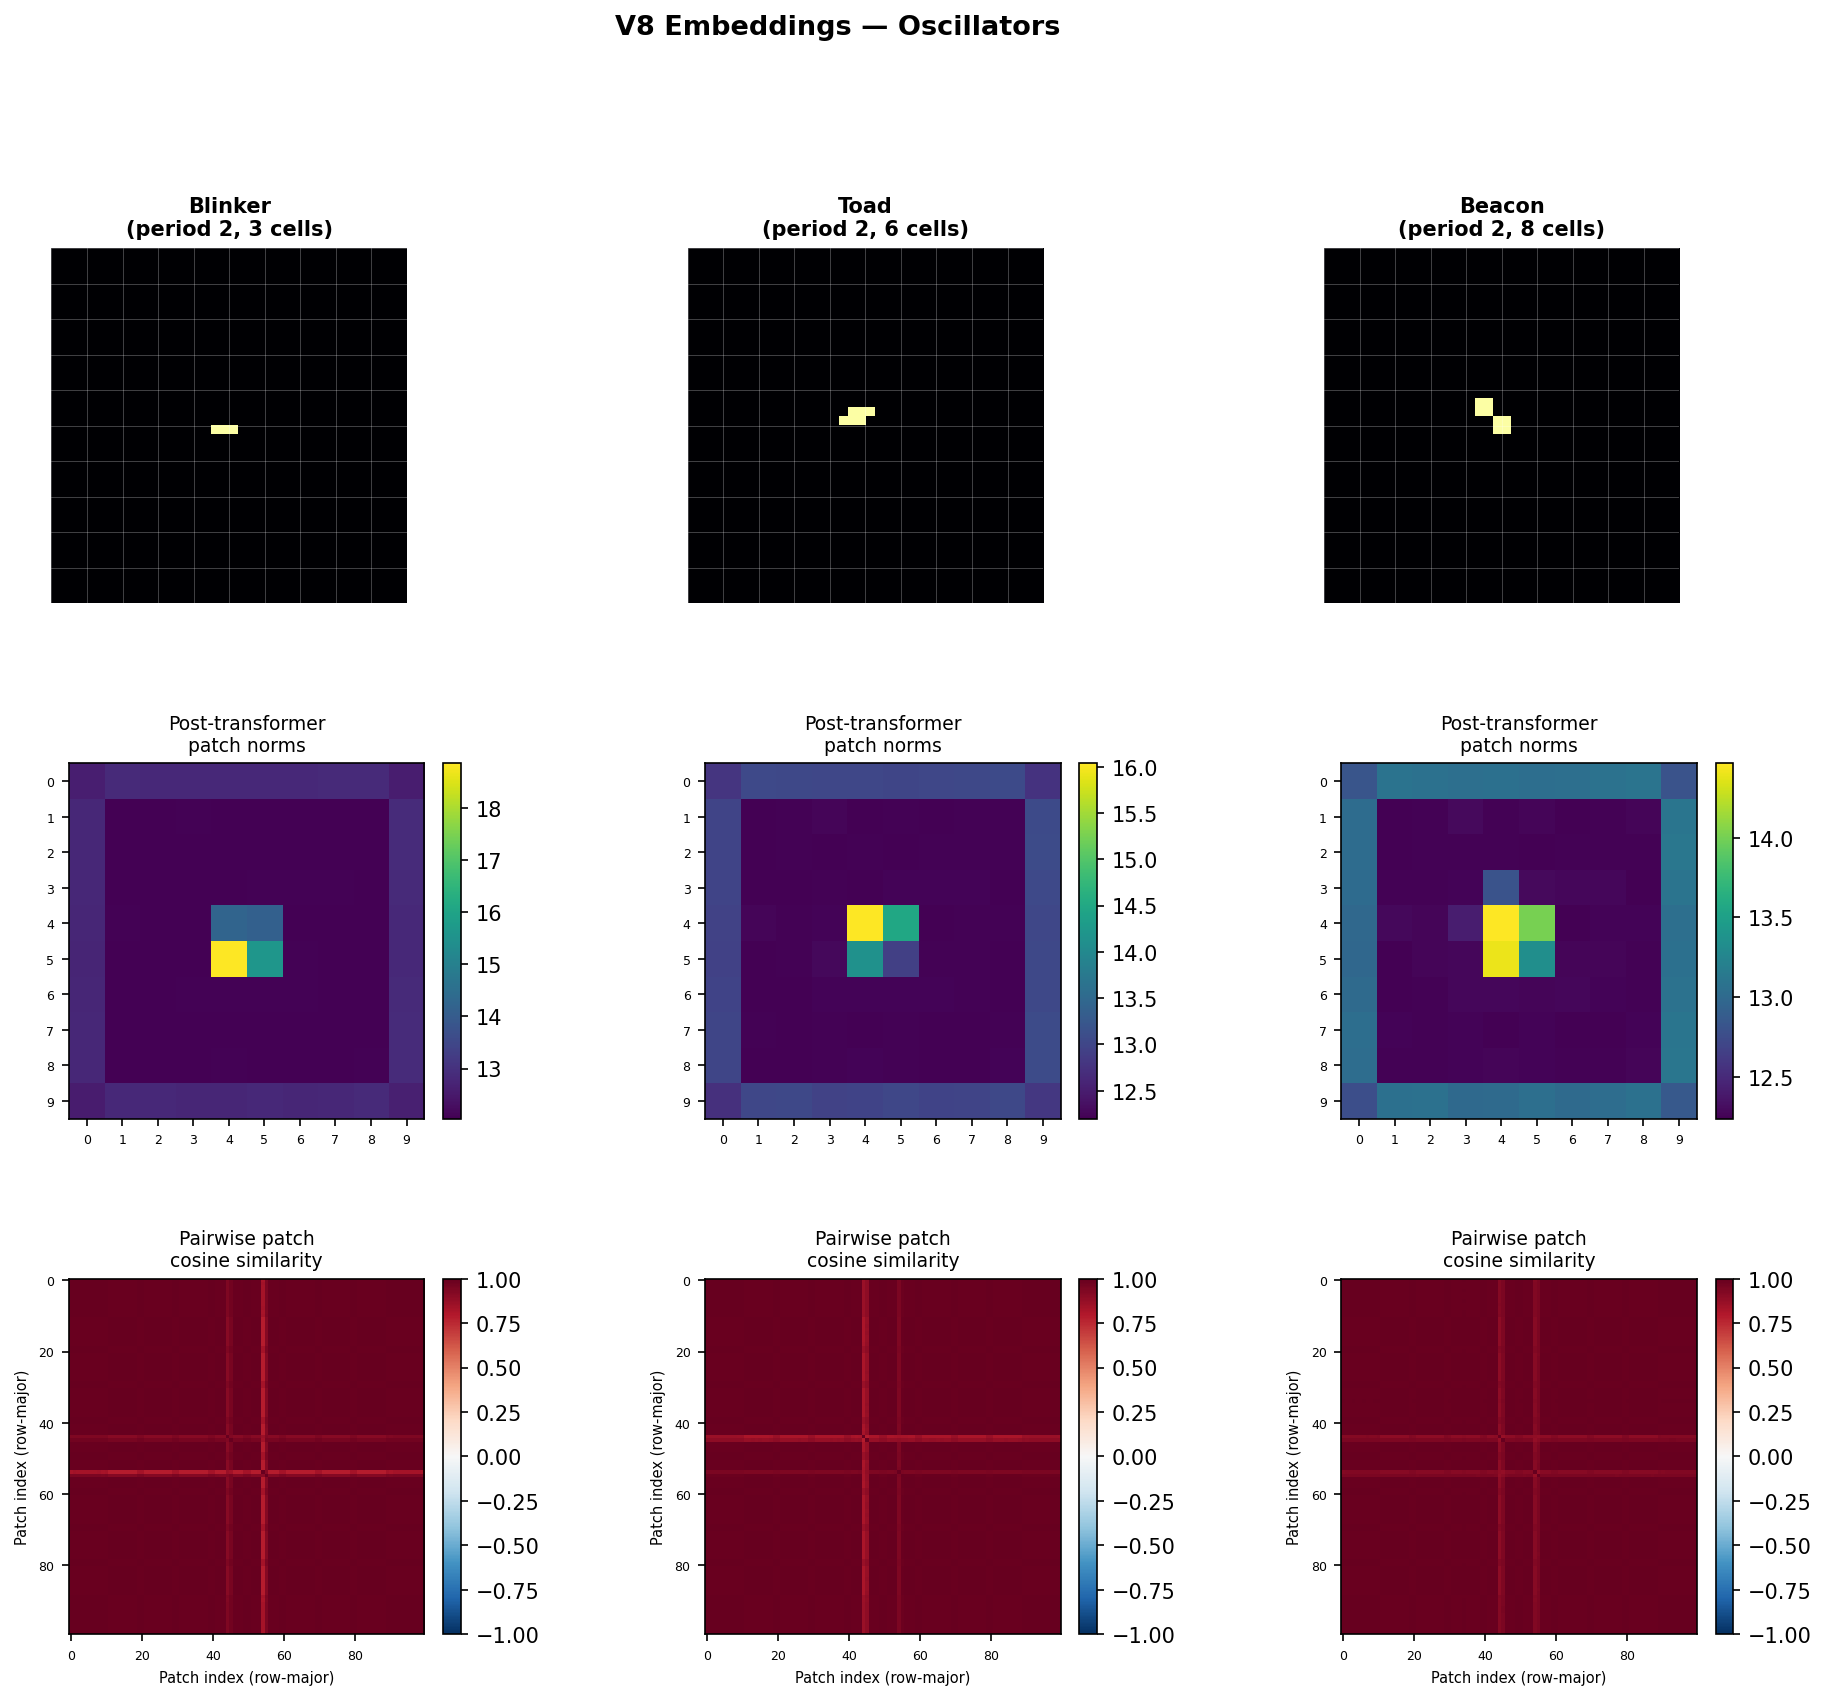
\includegraphics[width=\textwidth]{figures/gallery_v8_oscillators.png}
  \caption{V8 embeddings for three period-2 oscillators (blinker, toad,
  beacon). Top row: grid configuration. Middle row: post-transformer patch
  norm heatmap. Bottom row: $100\times100$ pairwise cosine similarity
  matrix. Sparse configurations produce a large, near-uniform block of
  mutually similar ``empty-patch'' embeddings, with only the 1--2 occupied
  patches standing apart.}
  \label{fig:gallery-oscillators}
\end{figure}

\begin{figure}[htbp]
  \centering
  \begin{subfigure}[t]{0.48\textwidth}
    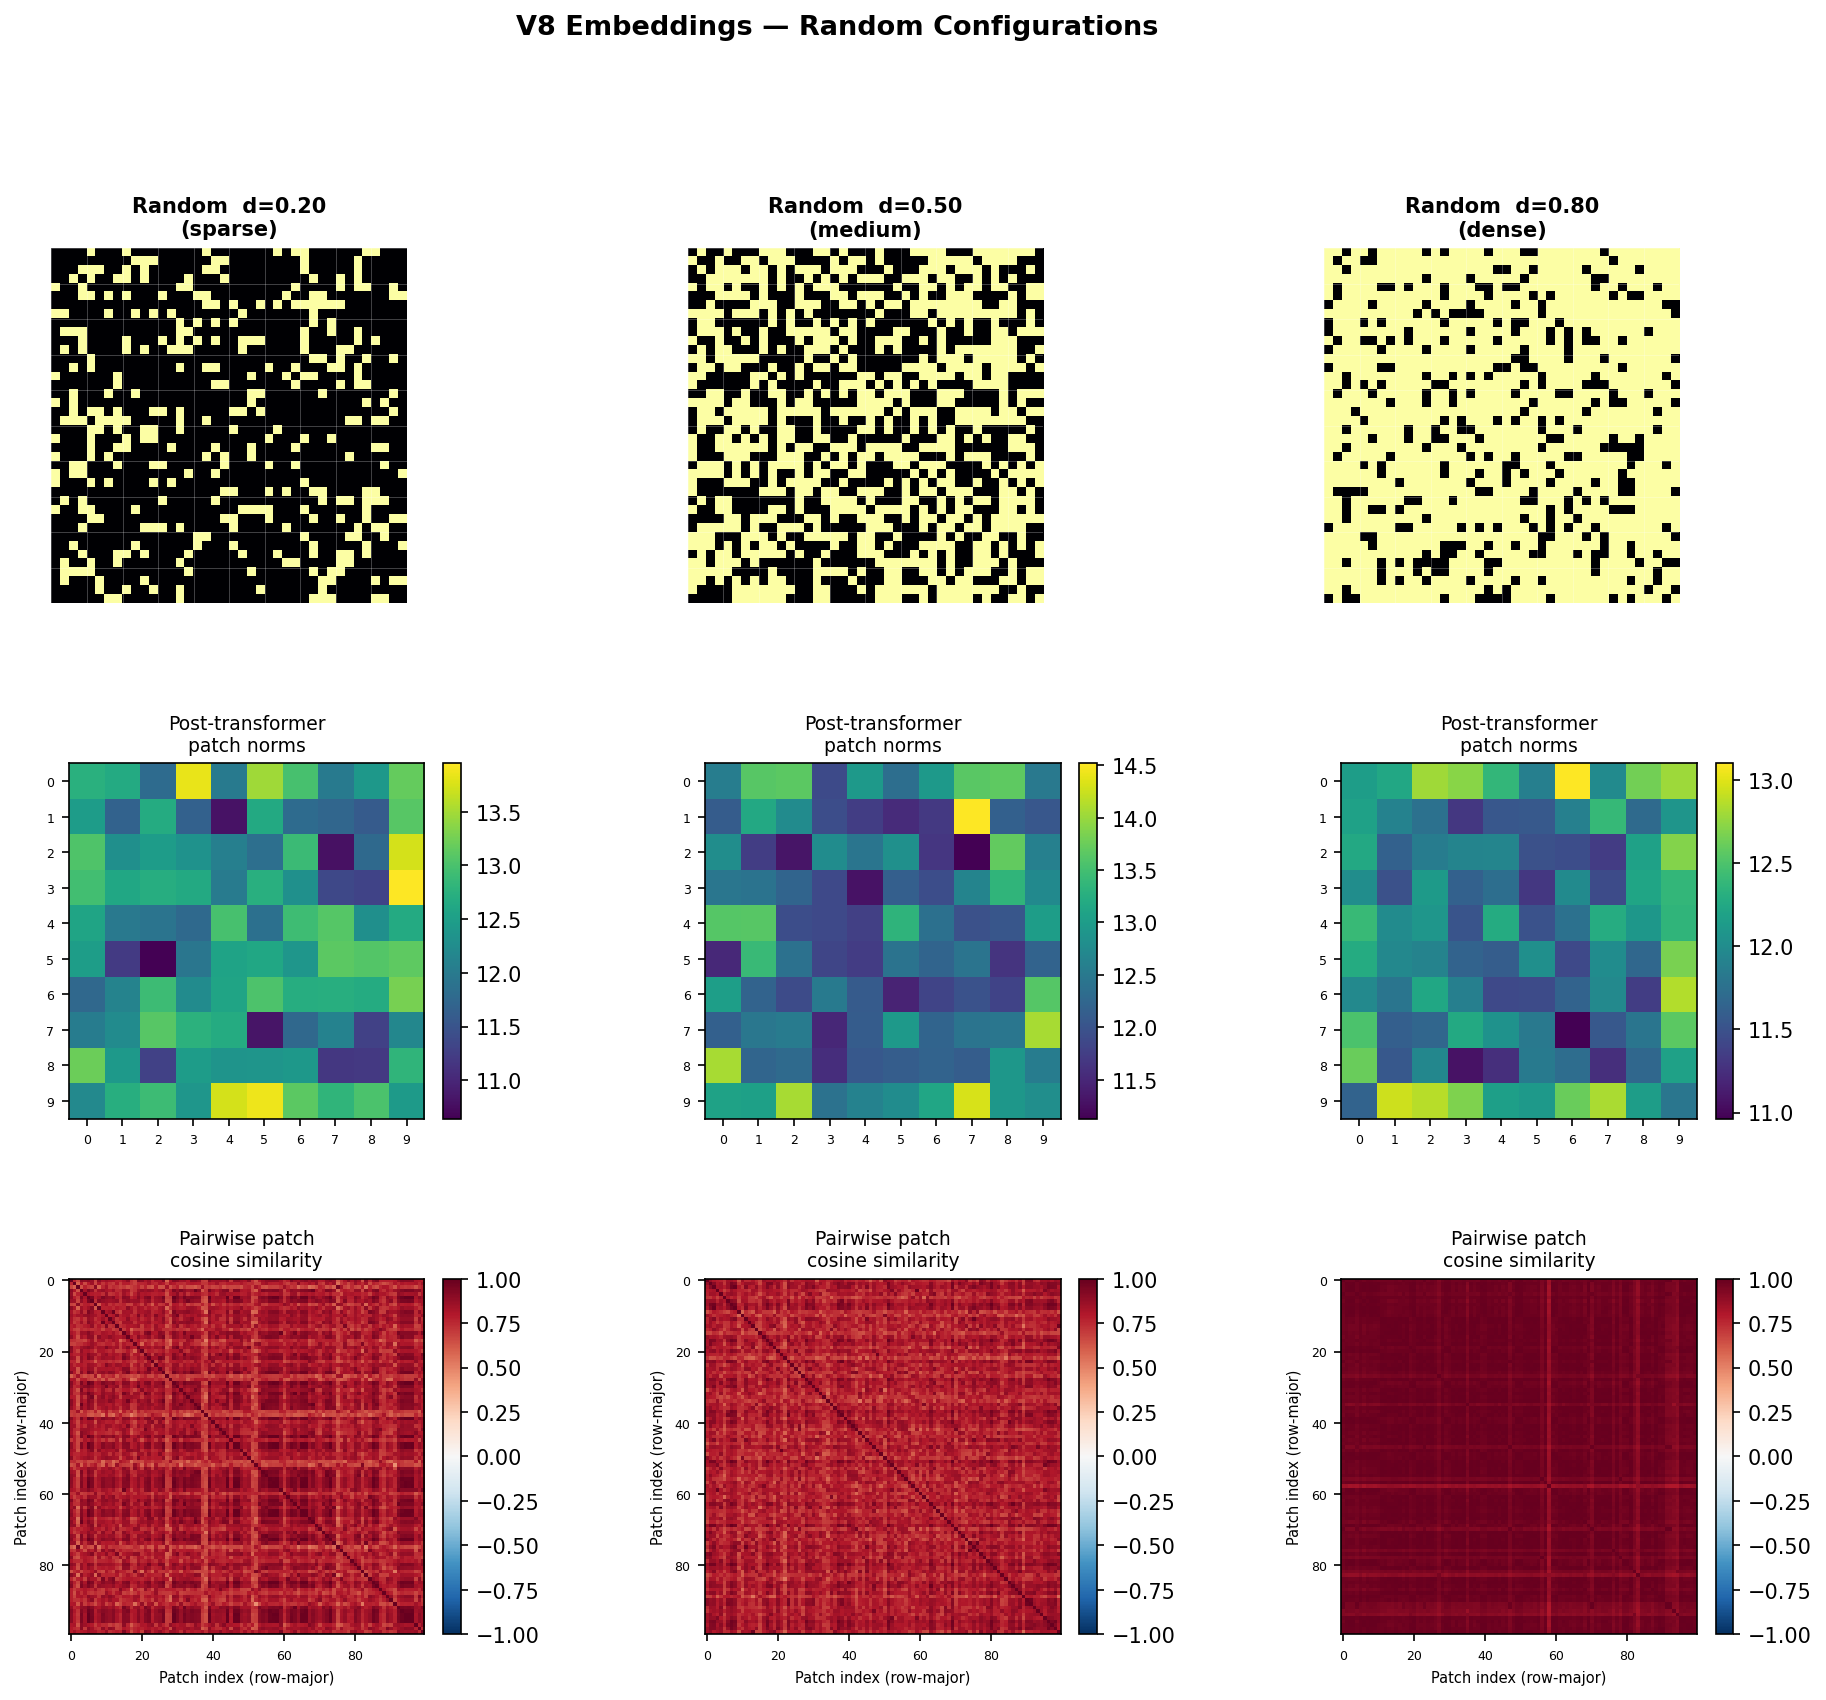
\includegraphics[width=\textwidth]{figures/gallery_v8_random.png}
    \caption{V8 (291K params)}
  \end{subfigure}
  \hfill
  \begin{subfigure}[t]{0.48\textwidth}
    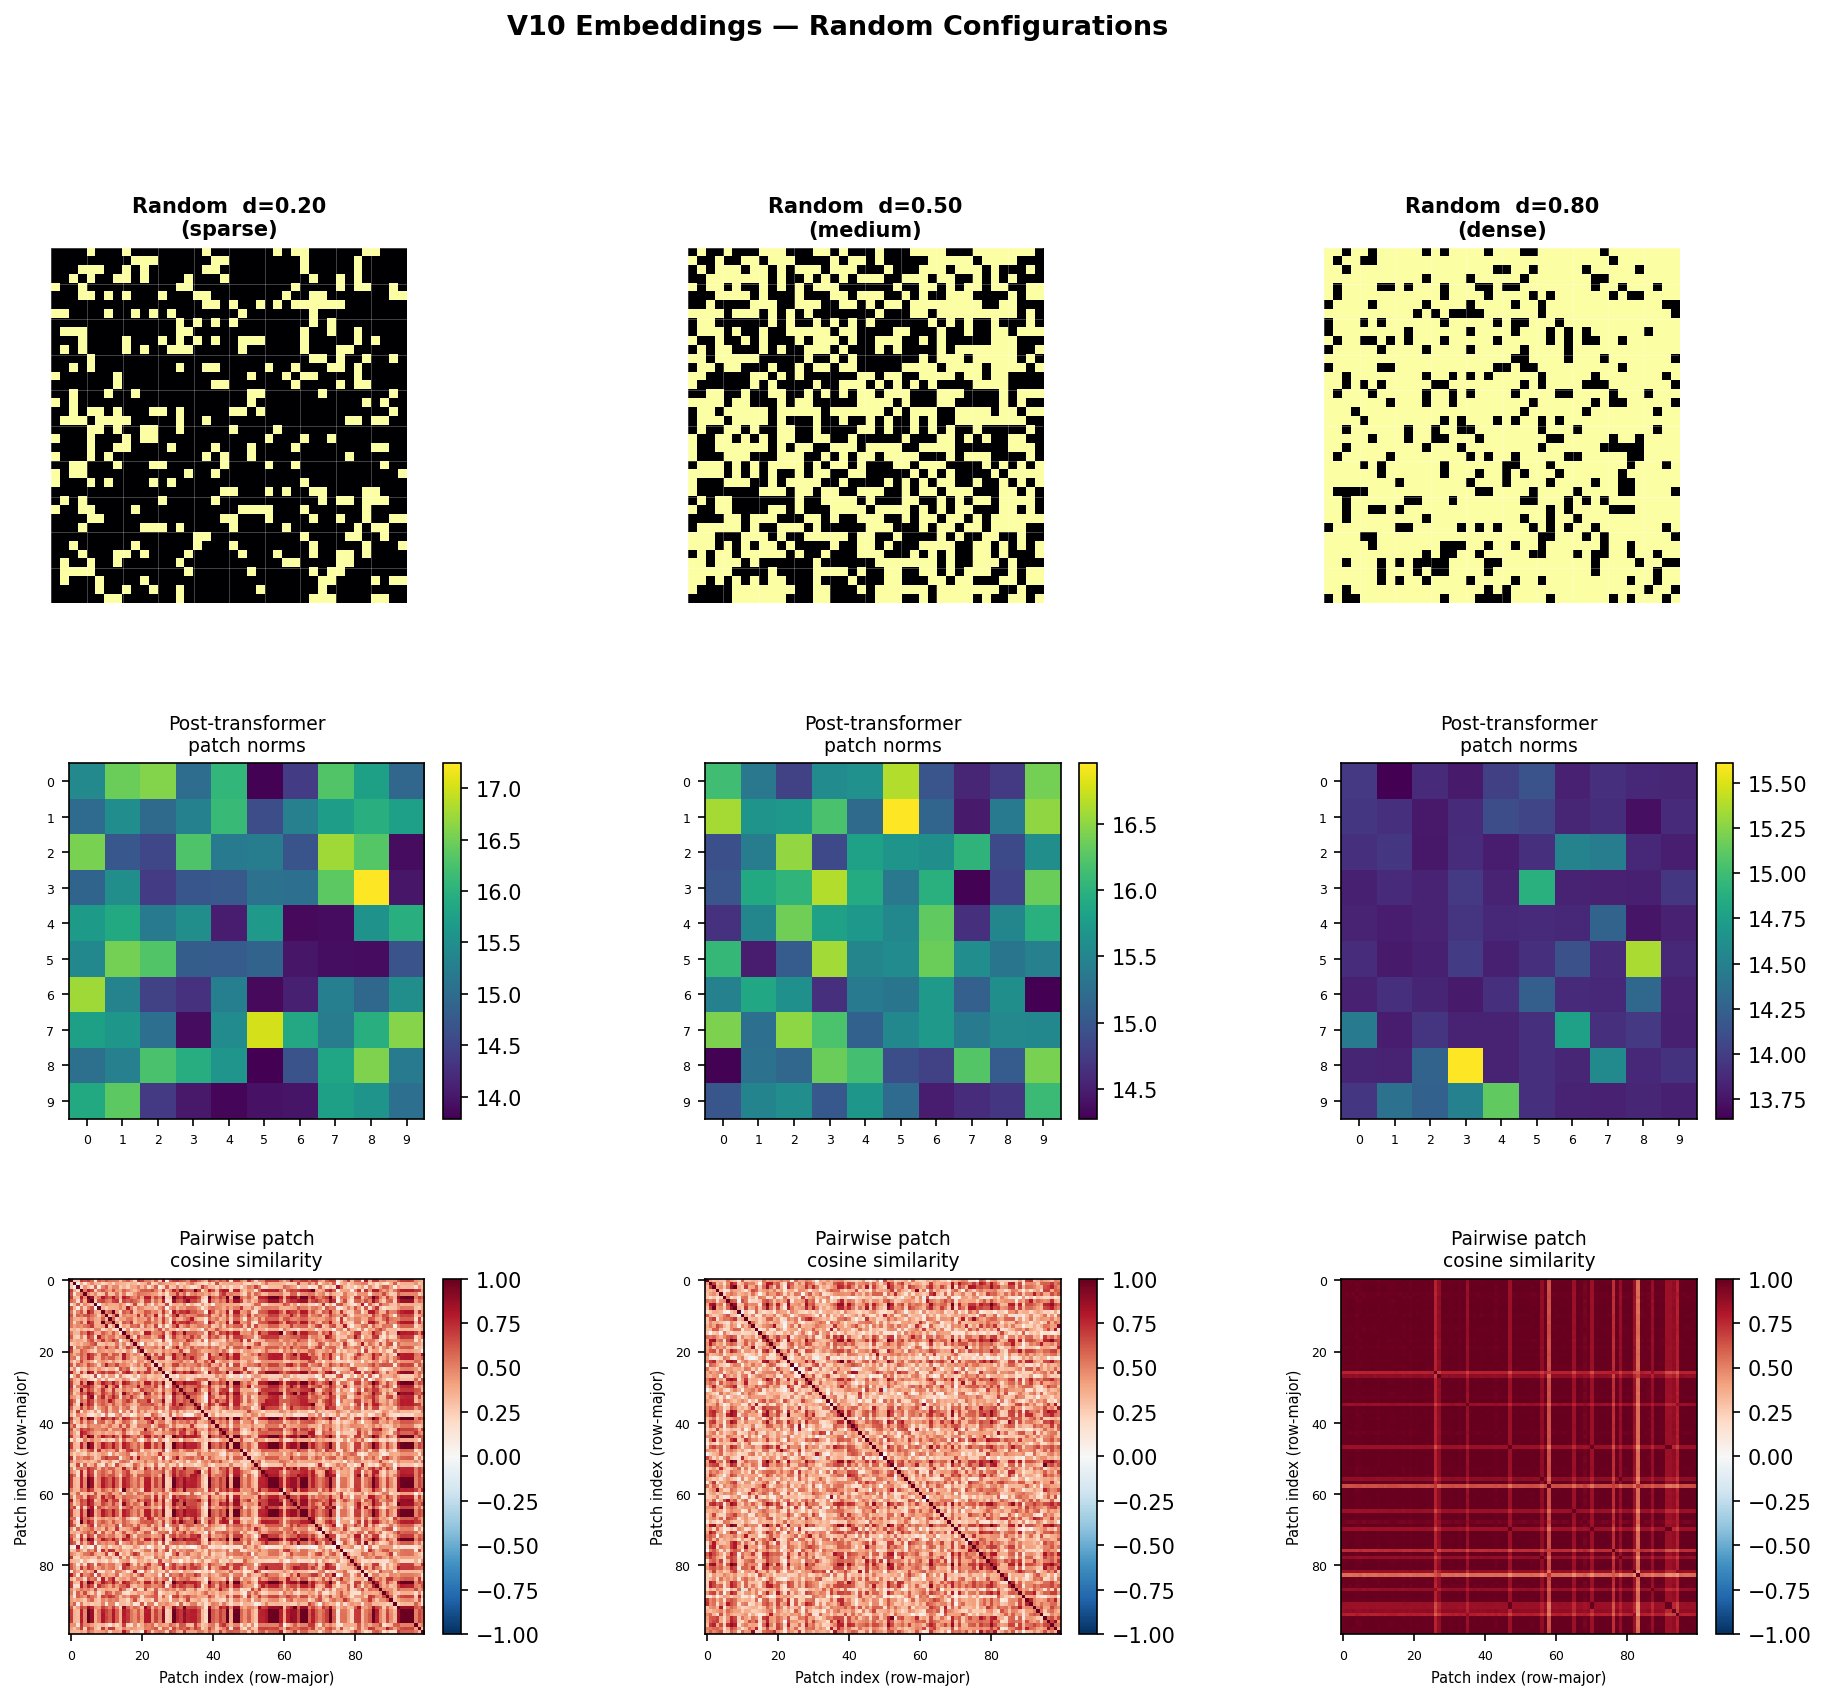
\includegraphics[width=\textwidth]{figures/gallery_v10_random.png}
    \caption{V10 (1.5M params)}
  \end{subfigure}
  \caption{Embeddings for random configurations at densities $0.20$, $0.50$,
  $0.80$ (left to right within each panel). As density increases, every
  patch carries genuine content, and the large ``empty-patch'' block seen
  in Figure~\ref{fig:gallery-oscillators} disappears, replaced by a more
  heterogeneous similarity structure.}
  \label{fig:gallery-random}
\end{figure}

Figure~\ref{fig:gallery-oscillators} shows that for sparse hand-placed
patterns, roughly 95--98 of the 100 patches are entirely empty and produce
near-identical embeddings (a large, uniformly high-similarity block in the
pairwise matrix), while the handful of occupied patches form a small,
distinct cluster. Figure~\ref{fig:gallery-random} shows this structure
eroding as density increases: at $d=0.80$, essentially every patch has
unique content, and the similarity matrix loses its block structure
entirely. This is a direct, visualizable signature of the sparse/dense
distinction that motivated the density-targeted fine-tuning in
Section~\ref{sec:training-evolution} (V8).

\subsection{Sensitivity to transformations}

We next measure how a patch's embedding changes under four families of
transformation applied to a fixed base configuration (glider, blinker, or
beacon): (i) $90^\circ/180^\circ/270^\circ$ rotation, (ii) horizontal/vertical
reflection, (iii) toroidal translation by 1 or 4 cells, and (iv) local
perturbation --- either flipping a single cell's state, or moving a single
live cell to an adjacent position. For each transformation we compute
$\Delta = \text{emb}(\text{transformed}) - \text{emb}(\text{original})$ per
patch, both pre- and post-transformer.

\begin{figure}[htbp]
  \centering
  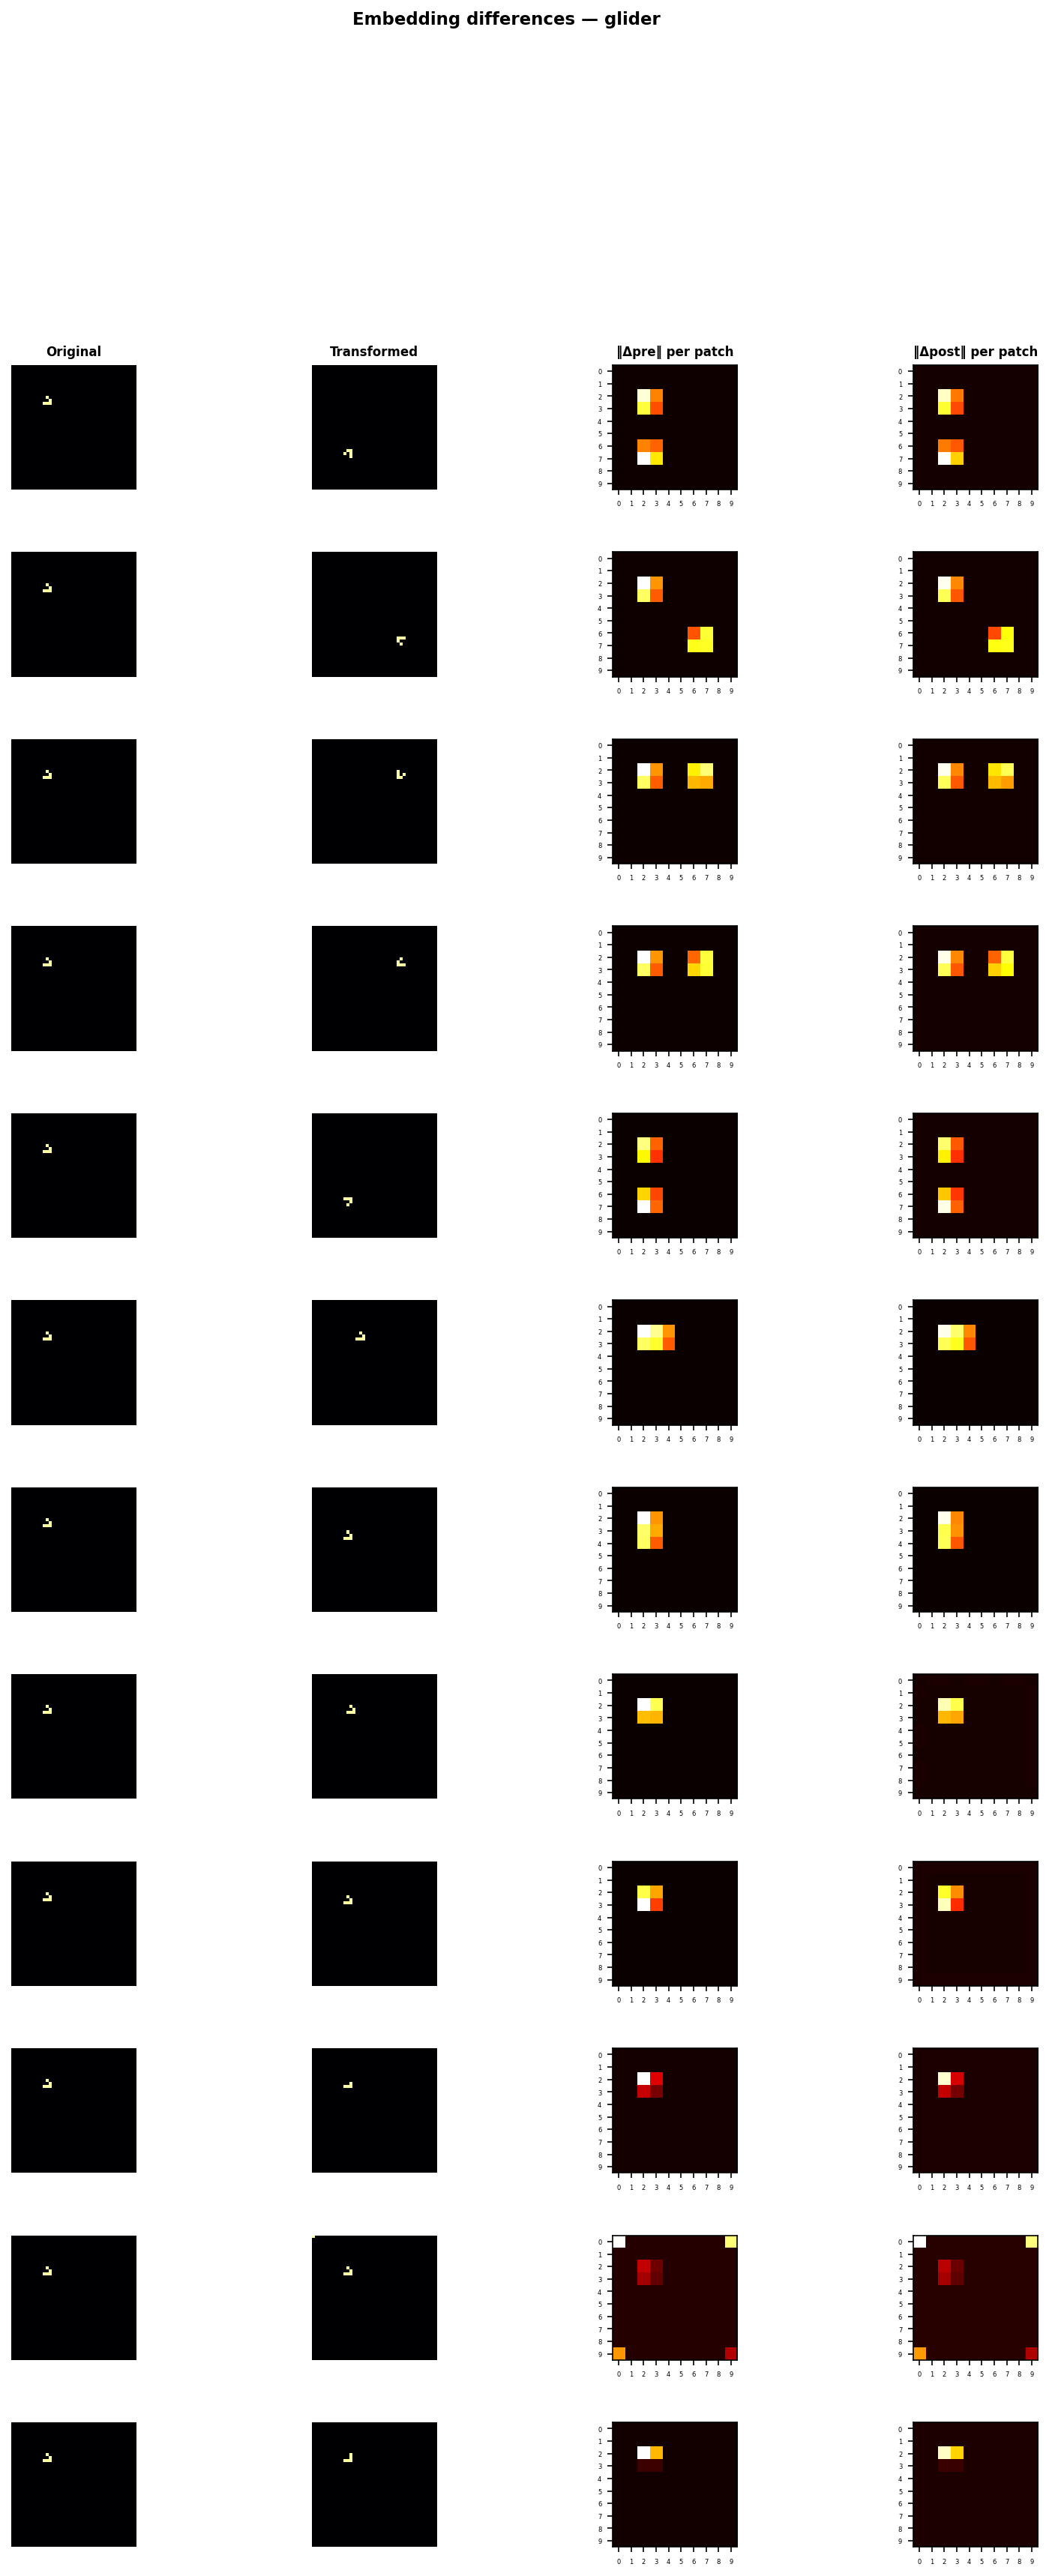
\includegraphics[height=0.75\textheight]{figures/embdiff_v8_deltanorms_glider.png}
  \caption{V8: per-patch embedding change $\|\Delta\|_2$ (pre- and
  post-transformer) for a glider under each transformation. Geometric
  transforms (rotation, reflection, coarse translation) perturb many
  patches at once because the pattern relocates to different absolute
  positions; single-cell perturbations affect only the one patch
  containing the perturbed cell.}
  \label{fig:embdiff-deltanorms}
\end{figure}

Table~\ref{tab:cosine-summary} (mean cosine similarity between original and
transformed post-transformer embeddings, averaged over all 100 patches)
quantifies the pattern visible in Figure~\ref{fig:embdiff-deltanorms}: sparse
patterns (glider) are nearly invariant to all transformations (cosine
similarity $\gtrsim 0.99$, since almost every patch is empty on both sides
of the transformation and empty patches encode almost identically
regardless of the grid's global content), while random grids show much
larger sensitivity to rotation, reflection, and coarse translation
($\approx 0.75$--$0.92$) because \emph{every} patch's absolute position
changes and the learnable positional embedding is position-specific, not
translation- or rotation-equivariant.

\begin{table}[htbp]
\centering
\begin{tabular}{lrrr}
\toprule
Transformation & Glider & Random ($d{=}0.35$) & Random ($d{=}0.65$) \\
\midrule
Rotate $90^\circ$        & 0.992 & 0.751 & 0.916 \\
Rotate $180^\circ$       & 0.991 & 0.744 & 0.909 \\
Flip horizontal          & 0.991 & 0.764 & 0.905 \\
Flip vertical            & 0.992 & 0.758 & 0.911 \\
Translate $+4$ cols      & 0.993 & 0.763 & 0.905 \\
Translate $+1$ col       & 0.996 & 0.780 & 0.924 \\
Cell flip (alive$\to$dead) & 0.9996 & --- & --- \\
Cell flip (dead$\to$alive) & 0.9988 & --- & --- \\
Cell move (1 step)         & 0.9987 & --- & --- \\
\bottomrule
\end{tabular}
\caption{Mean post-transformer cosine similarity between original and
transformed embeddings, V8. Sparse configurations are nearly invariant to
all transformations; dense random grids are substantially more sensitive to
geometric transforms, because the learnable absolute positional embedding
breaks exact translation/rotation equivariance.}
\label{tab:cosine-summary}
\end{table}

\subsection{Cross-transformation structure and geometry}

To ask whether different transformations perturb the embedding space in
\emph{similar directions}, we flatten each transformation's full
$\Delta \in \mathbb{R}^{100 \times d_{\text{model}}}$ vector and compute
pairwise cosine similarity across all transformations
(Figure~\ref{fig:embdiff-crosssim}). We additionally project the 100 patch
embeddings (original and every transformed version) into the top-2
principal components of the original configuration's embedding set
(Figure~\ref{fig:embdiff-pca}), to visualize how occupied patches move
through representation space under each transformation while the empty-patch
cluster remains essentially fixed.

\begin{figure}[htbp]
  \centering
  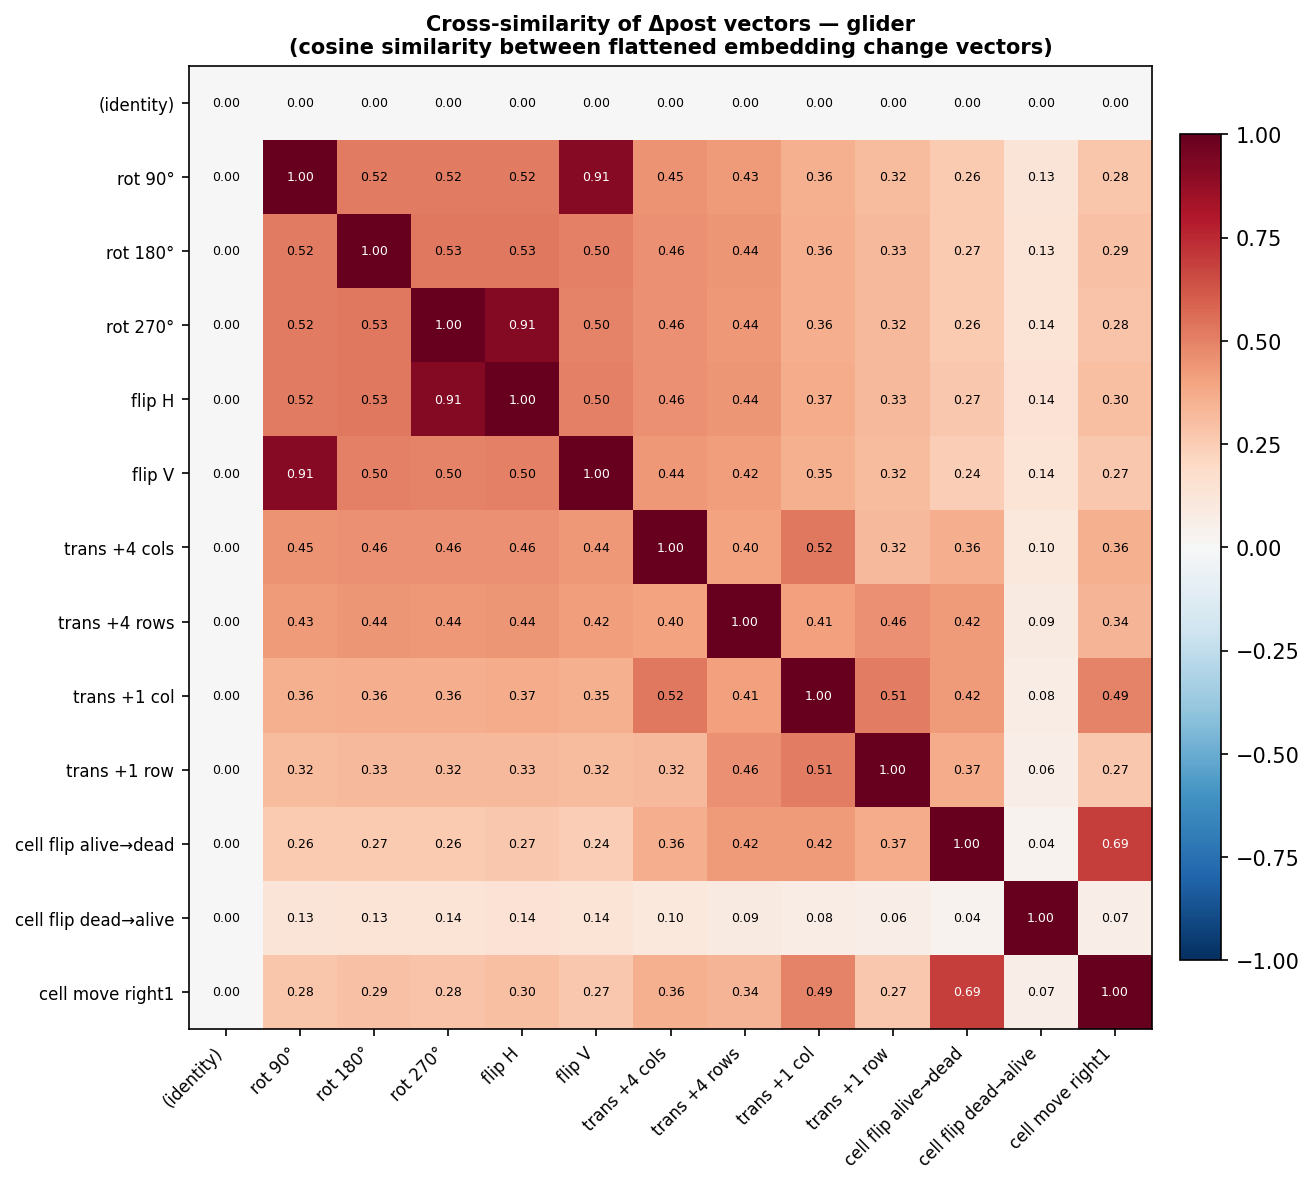
\includegraphics[width=0.7\textwidth]{figures/embdiff_v8_crosssim_glider.png}
  \caption{V8: cosine similarity between the flattened $\Delta_{\text{post}}$
  vectors of every pair of transformations (glider base pattern). Values
  near $1$ indicate two transformations perturb the embedding space in
  nearly the same direction; values near $0$ indicate unrelated
  perturbation directions.}
  \label{fig:embdiff-crosssim}
\end{figure}

\begin{figure}[htbp]
  \centering
  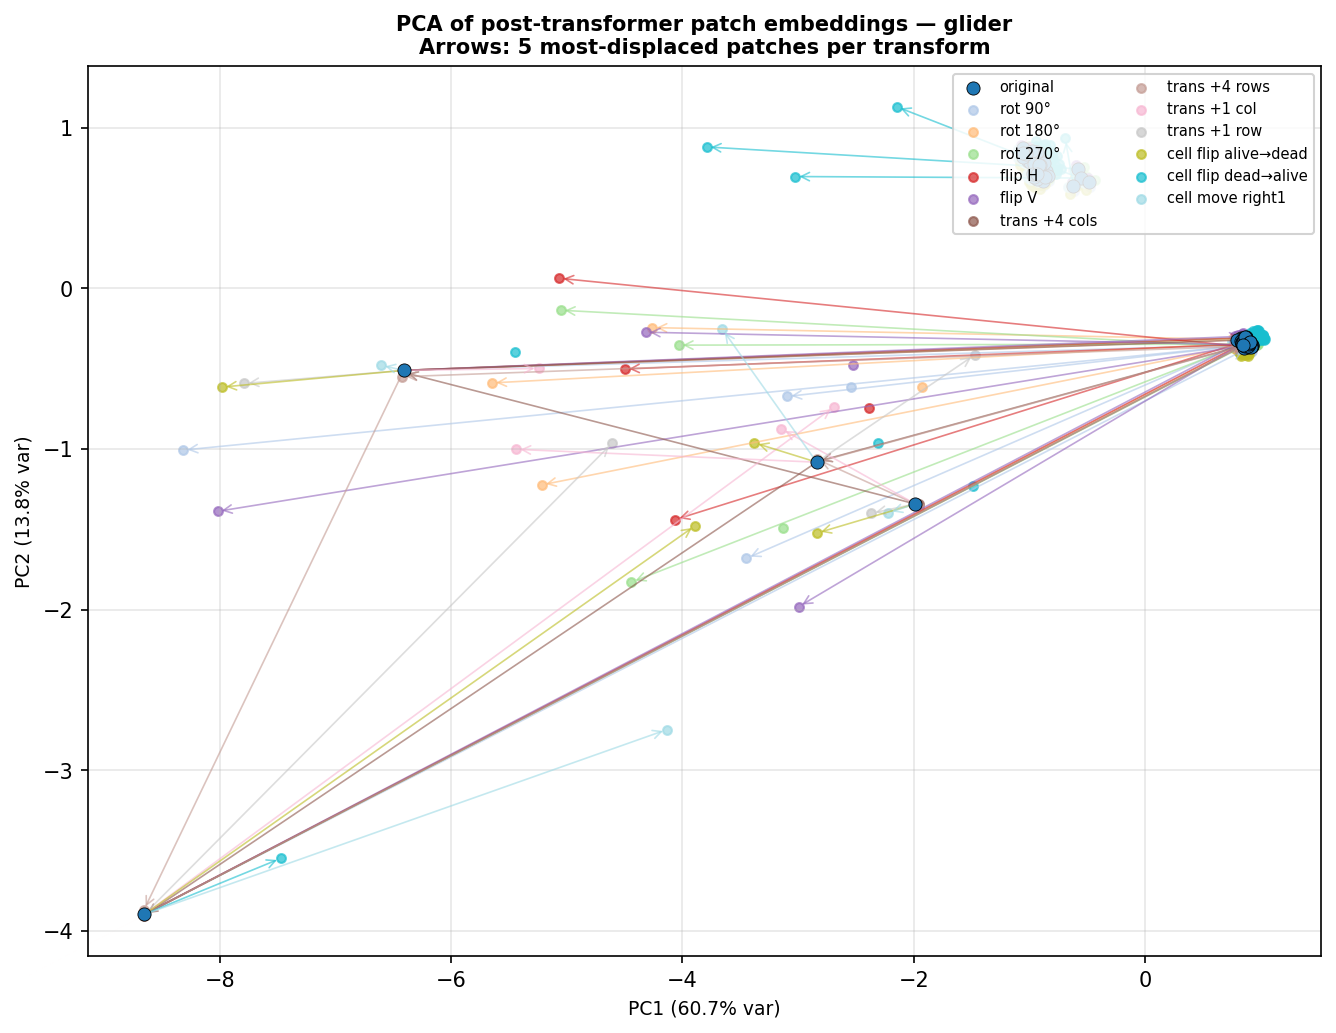
\includegraphics[width=0.7\textwidth]{figures/embdiff_v8_pca_glider.png}
  \caption{V8: PCA projection (fit on the original glider's 100 patch
  embeddings) of the embeddings under every transformation. The large
  central cluster is the $\sim$95 empty patches, essentially stationary
  across all transformations; arrows trace the 5 most-displaced patches per
  transformation, showing where the occupied-patch information moves to
  under each transform.}
  \label{fig:embdiff-pca}
\end{figure}

Qualitatively, geometric transformations (rotation, reflection) that share
the dihedral symmetry group used in data augmentation
(Section~\ref{sec:architecture}) tend to produce more mutually correlated
$\Delta$ vectors than translation does, consistent with the model having
been explicitly trained to be robust to (though not embedding-invariant
under) $D_4$ transformations, while translation invariance was never
encouraged during training.
